% Working paper. Master document (supersedes draft.md as of 2026-06-10).
% Target: BlackboxNLP @ EMNLP 2026 (direct deadline Jul 17, OpenReview). Swap
% \documentclass + preamble for the official ACL style file; everything below is
% template-agnostic.
% Build: pdflatex main && bibtex main && pdflatex main && pdflatex main
\documentclass[11pt]{article}
% Change "review" to "final" for the camera-ready version.
\usepackage[review]{acl}
\usepackage{times}
\usepackage{latexsym}
\usepackage[T1]{fontenc}
\usepackage[utf8]{inputenc}
\usepackage{microtype}
\usepackage{inconsolata}
\usepackage{booktabs}
\usepackage{array}
\usepackage{graphicx}
\usepackage{amsmath}
\usepackage{xcolor}
\newcommand{\todo}[1]{\textcolor{red}{[TODO: #1]}}
\newcommand{\pp}{\,\mathrm{pp}}
% Let URLs break at hyphens (the Llama 3.2 blog URL overflows its column otherwise).
\expandafter\def\expandafter\UrlBreaks\expandafter{\UrlBreaks\do\-}
% Leave short columns short instead of stretching glue into mid-column gaps
% (p7 left column and the appendix G column otherwise show holes).
\raggedbottom
% Pack floats tighter (appendix tables otherwise land one per mostly-empty page).
\setcounter{topnumber}{3}
\setcounter{dbltopnumber}{3}
\setcounter{totalnumber}{5}
\renewcommand{\topfraction}{0.95}
\renewcommand{\dbltopfraction}{0.95}
\renewcommand{\textfraction}{0.03}
\renewcommand{\floatpagefraction}{0.85}
\renewcommand{\dblfloatpagefraction}{0.85}
\graphicspath{{../figures/}}

\title{Leave the Sampler Alone:\\Truncation Changes Little Before a Model Collapses}
% Title alternatives:
%   The cliff is the model: temperature robustness and the limits of sampler tuning
%   Pick the model, not the sampler: temperature collapse is a model property
%   Temperature doesn't make LLMs wrong, it makes them ramble
\author{Anonymous}% double-blind: fill after acceptance

\begin{document}
\maketitle

\begin{abstract}
Truncation samplers such as top-$p$, min-$p$, and top-$n\sigma$ exist to prevent the
accuracy collapse of high-temperature sampling. Sampler evaluations compare one rule against another, mostly at temperatures where every
model has already collapsed. We ask whether it occurs in every model at the temperatures deployments use, from the
shipped defaults of 0.6 to 1.0 up to $T{=}1.3$. In a single controlled
pipeline, we run seven instruction-tuned models from five families across 8 sampler
arms, 4 quantization levels, and 2 tasks. At the shipped defaults, no truncation rule gains more than 3 points on any model
outside the Llama family (8 at the 95\% upper limit), and gains of 3 to 10 points appear
only at $T{=}1.3$, on the three models with the largest temperature drops outside Llama. Under plain temperature sampling at $T{=}1.3$,
Llama-3.1-8B and Llama-3.2-3B lose 34 to 41 accuracy points on GSM8K and MMLU-Pro, and
Llama-3-8B loses 17 on MMLU-Pro; no model outside the family loses more than 8. The
collapse is a termination failure. Generations derail midway and never reach an answer,
but when a model does produce a well-formed answer, it is as accurate as under greedy
decoding. A temperature ladder to $T{=}2.0$ on three models shows each collapsing at its own
temperature, with truncation samplers mattering only past it. Forcing one
off-distribution token into the context multiplies a fragile model's chance of drawing
another, so errors compound. Practitioners can screen a model for the collapse with fifty items and, if it passes,
leave the sampler alone.
\end{abstract}

\section{Introduction}

Sampling is the default decoding choice for deployed language models
\citep{shi2024decoding}, and truncation samplers exist to make it safe at high
temperature. They were designed for open-ended generation, where output variety is the
goal \citep{zhou2024decoding}, but they are now also evaluated on tasks with one
checkable answer. Min-$p$ reports accuracy gains over top-$p$ on GSM8K at high
temperature \citep{nguyen2024minp}, and top-$n\sigma$ reports accuracy maintained up to
$T{=}3.0$ \citep{tang2024topn}. Both results rest on the same premise, that raising the
temperature eventually ruins every model's accuracy and a good sampler limits the
damage. We test that premise at the temperatures deployments actually use and ask
\textbf{which models collapse in that range, and whether the sampler changes anything
before they do}.

There is a good reason to expect the collapse. At each step the decoder draws the next
token at random from the model's predicted distribution, and a temperature parameter
scales the randomness of the draw. Raising it
moves probability from the model's preferred tokens toward the rare ones in the tail of
the distribution, where the model's probability estimates are least reliable, so a
high-temperature draw can select a token that fits the context poorly
\citep{holtzman2020curious,hewitt2022truncation}. The selected token then becomes
context for every later step, and the continuation can degenerate into incoherent text.
Truncation samplers prevent this degeneration by deleting the tail of the distribution
before the draw, and the rules differ in where they cut.

The accuracy evidence has two problems. First, it generalizes from very few models.
Top-$n\sigma$'s results come from a single model, Llama-3-8B \citep{tang2024topn}, and
min-$p$'s main results from Mistral-7B \citep{nguyen2024minp}. Second, the gains are
demonstrated at temperatures of 1.5 to 3, while deployed systems ship defaults between
0.6 and 1.0 (Section~\ref{sec:setup}). 

Across nine instruction-tuned models from five families, run through one controlled
pipeline, only one family collapses in that range, and outside it the sampler is worth
at most a few points. The six models outside the Llama family hold their
accuracy at deployment temperatures ($T{\le}1.3$) under every sampler we test, staying
within 8 points of their low-temperature scores. Llama-3.1-8B and Llama-3.2-3B lose 34
to 41 accuracy points under plain temperature sampling, and Llama-3-8B, top-$n\sigma$'s
test model, loses 17 on the longer task.

Our contributions:
\begin{itemize}
  \item \textbf{A single-pipeline factorial study.} Seven instruction-tuned models, four
    GGUF quantization levels plus a BF16 anchor, eight decoding arms, and $T \in \{0.7,
    1.0, 1.3\}$, on GSM8K and MMLU-Pro ($N{=}50$ items, $K{=}3$ repetitions): 185{,}600
    generations, with item-clustered bootstrap CIs on every headline estimate.
  \item \textbf{Robustness is model-bound, and the fragility runs in one family.}
    Every collapse we observe inside the deployment band is a Llama: two generations collapse outright and a third
    loses 17 points on the longer task (Section~\ref{sec:modelbound}); on the robust models no truncation rule gains more than 3 points at the shipped
    defaults (8 at the 95\% upper limit) (Section~\ref{sec:spread}).
  \item \textbf{The collapse is a termination failure.} Among Llama's generations that reach a
    well-formed answer at $T{=}1.3$, accuracy matches greedy decoding on the same items.
    What changes is the probability of derailing into unparseable text mid-generation
    (Section~\ref{sec:degeneration}).
  \item \textbf{A cliff map from $T{=}1.3$ to $2.0$.} All three models we push to $T{=}2.0$ collapse, each at its own temperature. On GSM8K, Llama collapses by $T{=}1.5$, Qwen2.5
    by 1.7, and Gemma-3 by 2.0. Truncation shifts each cliff right, so the gains the sampler papers report sit
    past it (Section~\ref{sec:cliff}).
  \item \textbf{A mechanism signature.} A logit probe and a forced-token experiment
    locate the fragility after the first off-distribution token enters the context. One
    injected tail token multiplies Llama's chance of drawing another 2.3-fold, while no robust model's rises by more than $+0.0015$ per position, about a third of
    Llama's increase (Section~\ref{sec:mechanism}).
\end{itemize}

\section{Related work}
\label{sec:related}

\paragraph{Truncation samplers.}
Top-$k$ sampling draws from only the $k$ most probable tokens; it was introduced for
story generation, where likelihood-maximizing decoding produced generic and repetitive
text \citep{fan2018hierarchical}. \citet{holtzman2020curious} showed that a fixed $k$
fits poorly because the next-token distribution is sometimes peaked and sometimes flat,
and proposed nucleus sampling, which keeps the smallest set of tokens whose probabilities
sum to a target $p$. Min-$p$ keeps only the tokens whose probability is at least a set fraction of the top
token's, so the cut is tight where the model is confident and loose where it is
uncertain \citep{nguyen2024minp}.
Top-$n\sigma$ cuts in logit space instead, keeping tokens within $n$ standard deviations
of the top logit; temperature rescales all logits equally, so the surviving set does not
change with temperature \citep{tang2024topn}. Further refinements of the cut exist,
among them typical sampling and epsilon and eta sampling
\citep{meister2023typical,hewitt2022truncation}. \citet{welleck2020consistency} proved that top-$k$ and nucleus decoding can produce
sequences that never terminate even when the model itself always terminates, so
non-termination is a documented decoding failure. In contrast to the sampler papers, which
compare truncation rules against each other, we test whether the failure they all guard
against occurs at deployment temperatures at all.

\paragraph{Reproducibility of sampler gains.}
\citet{schaeffer2025minp} reanalyzed min-$p$ on nine models and 31 temperatures, giving
every sampler an equal number of hyperparameter settings, and found its reported gains
``largely indistinguishable'' from the other samplers'. A second variable in such a
comparison is the order in which temperature and truncation are applied. The order matters because the
truncation threshold is computed on whichever distribution the rule sees: applied before
temperature, the rule cuts the model's original, sharp distribution; applied after, it
cuts one that temperature has already flattened, so the same nominal setting keeps a
different set of tokens. We run the two chain orders as explicit arms
(Section~\ref{sec:setup}). \citet{zhou2024decoding} sweeps
decoding hyperparameters on open-ended generation with
quality and diversity metrics, while our tasks have one checkable answer.
\citet{shi2024decoding} compare decoding methods on closed-ended tasks and report that
the best method changes with the task and the model, and that quantization alters how
robust a model is to the choice; the comparison is again among methods, and it leaves
our premise question open.
\citet{song2024goodbad} documents per-model gaps between greedy decoding and sampling on
reasoning benchmarks and treats the gaps as evaluation noise to report; we treat the gap
as the object of study and trace it to a termination failure in one model family.

\paragraph{Robustness to decoding randomness.}
\citet{renze2024temperature} sampled temperatures from 0.0 to 1.6 on multiple-choice
problem solving and found no statistically significant effect on accuracy between 0.0 and
1.0. We replicate that null for most models, but per-model results show Llama-3.1-8B falling
just past $T{=}1.0$ while every other model holds (Section~\ref{sec:modelbound}).
The nearest study is \citet{grover2026reliability}, which also asks what makes a model
robust to decoding randomness and concludes that instruction tuning is the primary
determinant. Our data refine that conclusion. All nine of our models are instruction-tuned and one family still collapses, so instruction tuning cannot be the whole
answer. Their evaluation differs from ours in two respects that matter. Their sweep stops
at $T{=}1.0$, and the Llama collapse happens between 1.0 and 1.3; and their robust
models score 11 to 30\% on synthetic tasks, so there is little accuracy left to lose.
They also test no truncation samplers.
\citet{fastowski2025confidence} connect token-distribution entropy to temperature
sensitivity on factual question answering; our logit probe supports the link
(Section~\ref{sec:mechanism}), though size does not decide the outcome in our grid, where
Qwen3-1.7B holds and the larger Llama-3.1-8B collapses.

\section{Experimental setup}
\label{sec:setup}

The study is a factorial grid over four axes, model, quantization level, decoding arm,
and temperature, crossed with two tasks. Table~\ref{tab:design} lists the grid and the
smaller experiments around it. We call one model at one quantization level, on one task
at one temperature, a \emph{cell}; the eight decoding arms run inside every cell on the
same 50 frozen items. Every sampler comparison in the paper therefore holds the cell
fixed and varies the arm, and every temperature comparison holds the arm fixed and varies only the temperature. Everything outside the axes is pinned: one llama.cpp commit, each
model's official chat template rendered client-side, the native completion API, and
per-record seeds derived deterministically from the cell and arm. An accuracy difference
between two runs is then attributable to the axes, up to sampling noise that the
bootstrap below quantifies.

\begin{table*}[t]\centering
\caption{The experiments. Both tasks run in every row except Stratified (MMLU-Pro only,
fresh items); the BF16 anchor is Qwen3-4B only; the arms are listed under Decoding. Gen.\
counts graded generations, or prompts and continuations for the two probes (greedy runs
once per item; two Mistral prompts end before the injection point and are skipped).}
\label{tab:design}
\footnotesize\setlength{\tabcolsep}{3pt}\resizebox{\textwidth}{!}{\begin{tabular}{@{}llllrr@{}}
\toprule
Run & Models & Precision and engine & Configurations & $T$ & Generations \\
\midrule
Main grid & 7, from 5 families & Q8, Q6, Q4, Q3; llama.cpp & 8 & 0.7, 1.0, 1.3 & 185,600 \\
Temperature test & 6 more & Q8; llama.cpp & greedy, plain temp. & 0.7, 1.0, 1.3 & 6,000 \\
Flagged-model grid & 3 of the 6 & Q8; llama.cpp & 8 & 0.7, 1.0, 1.3 & 19,200 \\
Engine check & Llama-3.2, Llama-3.1, Qwen3-4B & BF16, INT8 (Transformers); F16, Q8 (llama.cpp) & greedy, plain temp. & 0.7, 1.0, 1.3 & 6,000 \\
Temperature sweep & Llama-3.1, Qwen2.5, Gemma-3 & Q8; llama.cpp & 4 & 1.3, 1.5, 1.7, 2.0 & 14,400 \\
Stratified subset & Llama-3.1, Qwen2.5, Gemma-3 & Q8; llama.cpp & greedy, plain temp. & 0.7, 1.0, 1.3 & 1,500 \\
\bottomrule
\end{tabular}
}
\end{table*}

\textbf{Decoding.} Each cell runs eight arms: a deterministic greedy anchor, plain
temperature sampling, and the four truncation rules of Section~\ref{sec:related}, each at
the setting its source paper uses or recommends: top-$p$ 0.95
\citep{holtzman2020curious}, top-$k$ 40 \citep{radford2019gpt2}, min-$p$ 0.05
\citep{nguyen2024minp}, top-$n\sigma$ 1.0 \citep{tang2024topn}.
Because the order of temperature and truncation changes which tokens survive
(Section~\ref{sec:related}), we pin temperature first across the truncation arms and add
two ablation arms that apply it last (the llama.cpp default) for top-$p$ and min-$p$, the
two rules whose surviving set depends on that order. Temperatures $T \in \{0.7, 1.0, 1.3\}$ span the deployment
band. The defaults that models and engines ship sit between 0.6 and 1.0 (Llama-3.1's
generation config sets 0.6, llama.cpp defaults to 0.8, the OpenAI and Anthropic APIs to
1.0),\footnote{Sources: Llama-3.1-8B-Instruct's \texttt{generation\_config.json},
llama.cpp's defaults, the OpenAI and Anthropic API references (July 2026).} so 0.7 and 1.0 bracket common practice and 1.3 sits just above it.
Every stochastic arm runs
$K{=}3$ repetitions per item; greedy decoding is deterministic, so $K{=}1$.

\textbf{Tasks.} We evaluate GSM8K, grade-school math word problems
\citep{cobbe2021gsm8k} (0-shot chain-of-thought with the prompt of Meta's Llama
evaluation suite \citep{meta2024llamaevals}, numeric exact
match), and MMLU-Pro, ten-option multiple-choice questions across 14 categories
\citep{wang2024mmlupro} (0-shot chain-of-thought, letter exact match), $N{=}50$ items each, a 512-token budget on GSM8K and 1024 on MMLU-Pro, with parsers
faithful to lm-eval-harness \citep{gao2023evalharness}. Both tasks require a chain of reasoning ending in one exactly checkable answer, which
keeps grading free of judge noise and leaves a long generation in which a derailment can
occur. The two tasks differ
in generation length, with MMLU-Pro's chains running roughly twice as long as GSM8K's, a
contrast Section~\ref{sec:cliff} uses to test whether longer generations fail earlier. Both tasks grade a generation by
parsing a final answer out of the generated text, so the parser decides how a generation
that never reaches an answer is graded. We log the parse path of every record: strict
when the pinned final-answer sentence is present (``The final answer is 26''; ``The
answer is (I)''), flexible when it is absent and the parser falls back to the last number
(GSM8K) or the last parenthesized option letter (MMLU-Pro), and failed when neither
exists, which grades as incorrect. Appendix~\ref{app:decomp} shows one generation per
path and checks the rule against markdown formatting. Every
contrast in the study compares runs on the same frozen items.

\textbf{Models and quantization.} The grid holds seven instruction-tuned models from five
model families: Llama-3.1-8B \citep{grattafiori2024llama}, Mistral-7B-v0.3
\citep{jiang2023mistral}, Qwen2.5-7B \citep{yang2024qwen25}, Qwen3-1.7B/4B/8B
\citep{yang2025qwen3} (thinking off; a thinking-on spot-check in
Appendix~\ref{app:thinking}), and Gemma-3-12B \citep{gemma2025gemma3}. A
follow-up temperature-only run adds two more Llama generations, Llama-3-8B
\citep{meta2024llama3} and Llama-3.2-3B \citep{meta2024llama32}
(Section~\ref{sec:modelbound}). Each model runs at four quantization levels
(Q8\_0, Q6\_K, Q4\_K\_M, Q3\_K\_M), all imatrix GGUF conversions from a single provider
so the quantization axis is not confounded by the conversion
recipe. A BF16 anchor on Qwen3-4B matches Q8 within noise, which lets Q8 stand in for
full precision.

\textbf{Statistical inference.} All confidence intervals come from a nonparametric
bootstrap ($B{=}2000$; 5000 for the contrasts of Appendix~\ref{app:bound}) clustered
on task items: we resample the 50 items rather than
individual generations, because the $K{=}3$ repetitions of one item share that item's
difficulty and treating them as independent would understate the uncertainty. Where a
comparison shares items across its two sides, which is everywhere in the grid, the
bootstrap is paired.

\textbf{Hardware and reproducibility.} The study totals about 205{,}000 graded
generations (Table~\ref{tab:design}). Hardware and the pinned llama.cpp commit are in Appendix~\ref{app:repro}; model-file
hashes are in the repository's \texttt{DOWNLOADS.md}.

\section{Results}

\subsection{The collapse is model-bound}
\label{sec:modelbound}

We begin with plain temperature sampling and no truncation, because the accuracy a
model loses when its full distribution is sampled at a higher temperature is exactly the
failure the truncation samplers of Section~\ref{sec:related} exist to prevent. Figure~\ref{fig:collapse} plots the drop
from $T{=}0.7$ to $T{=}1.3$, pooled over quantization levels, and
Table~\ref{tab:collapse} gives the exact values.

\begin{figure*}[t]
\centering
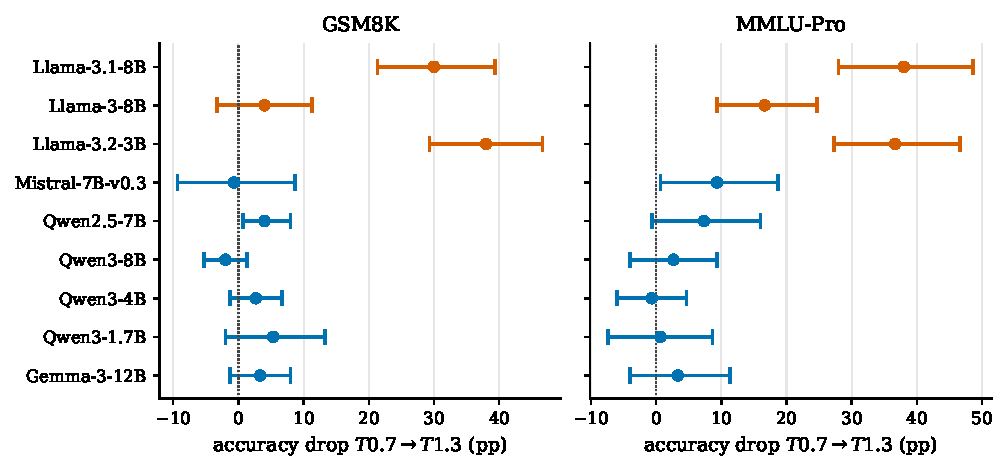
\includegraphics[width=0.72\textwidth]{fig1_collapse}
\caption{The pure-temperature collapse is model-bound: accuracy drop $T0.7 \to T1.3$,
points with 95\% item-clustered bootstrap CIs.}
\label{fig:collapse}
\end{figure*}

\begin{table}[t]
\centering
\caption{Plain-temperature accuracy drop $T0.7 \to T1.3$ (pp, 95\% item-clustered
bootstrap CIs; pooled over quantization levels, five for Qwen3-4B including BF16) and
sampler max$-$min accuracy spread at
$T{=}1.3$ (pp; CIs in Figure~\ref{fig:spread}).}
\label{tab:collapse}
\footnotesize
\setlength{\tabcolsep}{3.5pt}
\begin{tabular}{llrc}
\toprule
Model & Task & \multicolumn{1}{c}{drop [95\% CI]} & spread \\
\midrule
Llama-3.1-8B & GSM8K & $\mathbf{+34.0}$ [28.5, 39.7] & 36.7 \\
 & MMLU-Pro & $\mathbf{+40.8}$ [31.8, 50.3] & 41.8 \\
Mistral-7B-v0.3 & GSM8K & $+3.5$ [$-1.2$, 8.5] & 5.3 \\
 & MMLU-Pro & $+8.0$ [3.5, 13.2] & 10.0 \\
Qwen2.5-7B & GSM8K & $+4.0$ [1.2, 7.3] & 3.8 \\
 & MMLU-Pro & $+4.8$ [1.3, 8.8] & 5.7 \\
Gemma-3-12B & GSM8K & $+2.0$ [$-0.0$, 4.8] & 3.3 \\
 & MMLU-Pro & $+3.7$ [0.2, 7.7] & 5.8 \\
Qwen3-8B & GSM8K & $+0.5$ [$-1.5$, 2.6] & 1.8 \\
 & MMLU-Pro & $+1.0$ [$-2.4$, 4.8] & 3.5 \\
Qwen3-4B & GSM8K & $+2.1$ [0.4, 3.9] & 1.3 \\
 & MMLU-Pro & $+0.7$ [$-1.0$, 2.5] & 1.7 \\
Qwen3-1.7B & GSM8K & $-0.3$ [$-3.8$, 3.0] & 3.2 \\
 & MMLU-Pro & $+0.7$ [$-3.4$, 5.0] & 5.5 \\
\bottomrule
\end{tabular}
\end{table}

The models form a gradient rather than two groups: the Qwen3 family drops at most 2\,pp,
Qwen2.5, Gemma, and Mistral drop 2 to 8\,pp with at least one task CI excluding zero,
and Llama drops 34 to 41\,pp. Llama's drop begins inside the shipped band: from
$T{=}0.7$ to 1.0 it loses 8\,pp on MMLU-Pro and its run-to-cap rate doubles
(Appendix~\ref{app:decomp}). Three controls rule out the obvious confounds. Accuracy
headroom does not explain the collapse: Qwen3-1.7B scores 74\% on GSM8K, close to
Llama's 78\%, and does not collapse. Model age does not explain it either, since
Mistral-7B-v0.3 predates Llama-3.1 and is robust. The stratified MMLU-Pro replication reproduces the pattern on fresh items, giving Llama $+43.3\,$pp [31.3, 55.3], Qwen2.5 $+6.0$, and
Gemma $+7.3$.

A single collapsing checkpoint could still be a quirk of that release rather than a
family trait, so a follow-up run repeats the pure-temperature axis on two more Llama
generations, Llama-3-8B and Llama-3.2-3B (Q8, same frozen items, $K{=}3$; drops and accuracy levels in
Appendix~\ref{app:lineage}).
Llama-3.2-3B collapses
like Llama-3.1-8B ($+38.0\,$pp on GSM8K, $+36.7$ on MMLU-Pro)
and with the same degeneration signature as Section~\ref{sec:degeneration}.
Llama-3-8B sits between the two: a null on GSM8K but
$+16.7\,$pp on MMLU-Pro, the longer task, a
larger drop than any non-Llama model shows in Figure~\ref{fig:collapse}. Three Llama
generations produce the three largest MMLU-Pro drops in the study. The fragility recurs
across the family's releases, and what sets it apart from the other four families is the open question of Section~\ref{sec:discussion}. One family
collapses inside the deployment band, and no model outside it loses more than 8 points.

\subsection{The sampler changes little before the cliff}
\label{sec:spread}

This subsection holds temperature at $T{=}1.3$, the top of the deployment band, and
varies the sampler. The maximum minus minimum accuracy across the seven
stochastic sampler arms is 1.3 to 10.0\,pp on every robust model
(Table~\ref{tab:collapse}, spread column; per-arm accuracy grids in
Appendix~\ref{app:grids}), and even those numbers
overstate the axis, because the maximum and minimum of seven noisy estimates drift apart
by chance. On Llama the spread is not sampler noise: under plain temperature it has already
collapsed at $T{=}1.3$ and under top-$n\sigma$ it has not (Section~\ref{sec:cliff}), so
the spread measures how much of the collapse each rule prevents.

We therefore compare each of the six truncation arms with plain temperature directly:
for each model, task, and temperature, the paired accuracy difference on the same items,
with an item-clustered bootstrap CI (all
contrasts in Appendix~\ref{app:bound}; a GEE over the full grid, clustered on item,
reproduces every interval to within 0.6\,pp). At $T{=}0.7$ and 1.0, the temperatures
models ship with, no arm gains more than 3.3\,pp on any robust model, no pointwise upper 95\% limit
exceeds 7.5\,pp (a simultaneous bound on the largest gain over all 144 contrasts is 7.8),
135 of 144 point estimates lie within 3\,pp of plain temperature, and 6 intervals
exclude zero (2 above, 4 below), the number chance alone gives. At $T{=}1.3$, 22 of 72 contrasts lie above zero, all on Mistral, Qwen2.5, and Gemma-3,
the three non-Llama models with the largest temperature drops, with gains of 3 to
10\,pp, largest on the longer task; no Qwen3 contrast leaves zero at any temperature. On the robust models truncation is worth nothing at the shipped defaults and a few
points once a model has begun to collapse; on Llama the hardest-cutting rules are
already worth 6 to 11\,pp on MMLU-Pro at $T{=}1.0$ (Appendix~\ref{app:bound}), where
its collapse has begun.

Chain order changes accuracy by at most 4\,pp on the robust models at $T \le 1.0$ and by
up to 7\,pp on Mistral at $T{=}1.3$; on Llama, truncating before temperature scaling is
more protective at $T{=}1.3$
(top-$p$ 64\% $\to$ 73\% on GSM8K), as the threshold mechanics of
Section~\ref{sec:related} predict (both orders in Appendix~\ref{app:tlast}).

\subsection{The collapse is degeneration, not wrong answers}
\label{sec:degeneration}

This subsection works under plain temperature sampling throughout. An accuracy drop
can come from two failures: completed answers that are wrong, or generations that never
reach an answer. The parse path that Section~\ref{sec:setup} logs for every record
separates the two, so we decompose Llama's collapse along it
(Figure~\ref{fig:decomposition}; full decomposition and example outputs in
Appendix~\ref{app:decomp}).

\begin{figure*}[t]
\centering
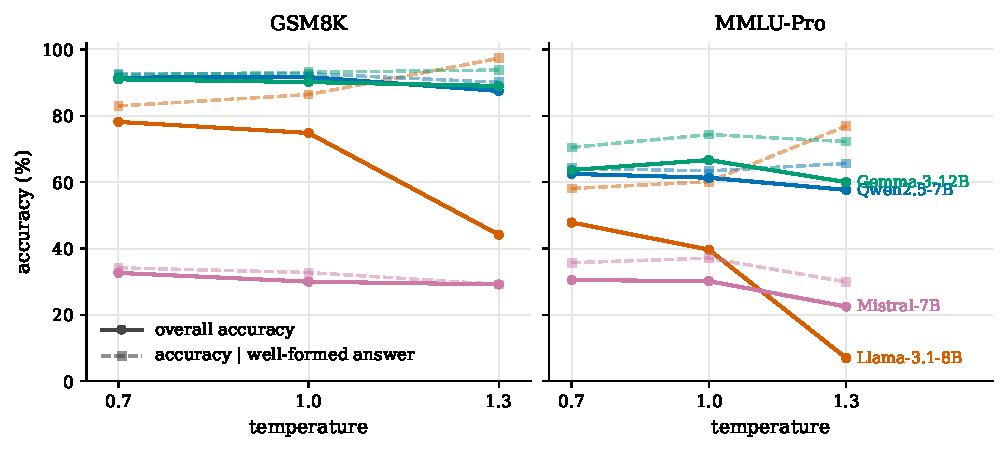
\includegraphics[width=0.78\textwidth]{fig2_decomposition}
\caption{Overall accuracy (solid) versus accuracy among well-formed, strict-parsed answers
(dashed) under plain temperature sampling; four models spanning the robustness gradient
(the three Qwen3 models are flat and omitted for legibility). The dashed lines never fall: among well-formed answers accuracy holds, and Llama's rise
is survivorship (Section~\ref{sec:degeneration}).}
\label{fig:decomposition}
\end{figure*}
Nearly all of the drop is the second failure. At $T{=}1.3$, 53.8\% of Llama's GSM8K
generations and 89.2\% of its MMLU-Pro generations derail into token-level noise and run
to the token cap. Among the generations that do produce a well-formed final answer (a strict parse: the pinned final-answer sentence is present), Llama still scores
97.3\% on GSM8K at $T{=}1.3$. That number needs one correction. Survival is selective, because easier items produce shorter generations and
shorter generations have less room to derail, so the 97.3\% is measured on an
easier-than-average set of items. The right comparison for it is greedy decoding on those same surviving items at the
same quantization level, which scores 97.3\%, against 78.0\% on all items. Among the generations that finish, then, accuracy at $T{=}1.3$ matches greedy decoding
(97.3 vs.\ 97.3\% on GSM8K; 76.9 vs.\ 78.8\% on MMLU-Pro).

The two tasks report one failure differently: degenerate text almost always contains a
number, so GSM8K's last-number fallback grades a derailed generation as a wrong answer,
while MMLU-Pro's letter parser reports a parse failure. Temperature does not raise Llama's rate of wrong answers; it raises the rate of
generations that never reach one.

\subsection{The cliff map: robustness is cliff location}
\label{sec:cliff}

To see whether the robust models also collapse at higher temperature, we extend the
temperature axis to $T \in
\{1.3, 1.5, 1.7, 2.0\}$ on three models spanning the gradient of Figure~\ref{fig:collapse}:
Llama-3.1-8B, Qwen2.5-7B, and Gemma-3-12B (Q8, both tasks, $N{=}50$, $K{=}3$).
Figure~\ref{fig:cliff} and Table~\ref{tab:cliff} give the trajectories and the drops
against each model's own $T{=}0.7$ anchor. Every model turns out to have
a cliff, and what distinguishes the models is where it sits. Calling the cliff the first rung at which a model loses more than half its $T{=}0.7$
accuracy, the three models collapse on GSM8K in their Figure~\ref{fig:collapse} order:
Llama at 1.5, Qwen2.5 at 1.7, and Gemma at 2.0. At $T{=}1.5$ the CI of Llama's drop does not overlap the other two models', and at
$T{=}1.7$ Qwen2.5's does not overlap Gemma's. Within each model the cliff
sits earlier on MMLU-Pro, the task with roughly twice the generation length, as expected if the risk is per token and accumulates over a longer generation. There Llama has already collapsed at
$T{=}1.3$, and Qwen2.5 and Gemma fall together at $T{=}1.5$.

Truncation shifts the cliff right in order of tail-cutting strength: top-$p$ moves the
cliff about 0.2 higher, min-$p$ holds 70\% at $T{=}1.5$ on Llama GSM8K where plain
temperature is at 9\%, and top-$n\sigma$ is flat to $T{=}2.0$ on all three models. The strict-parse rate tracks accuracy almost one-to-one along the
whole ladder, so the accuracy cliff coincides with the degeneration cliff. This reconciles the sampler papers with Section~\ref{sec:spread}: min-$p$ and
top-$n\sigma$ are validated at temperatures of 1.5 to 3 \citep{nguyen2024minp,tang2024topn},
past every model's deployment range, where their gains are real (Appendix~\ref{app:hight}). 

\begin{figure*}[t]
\centering
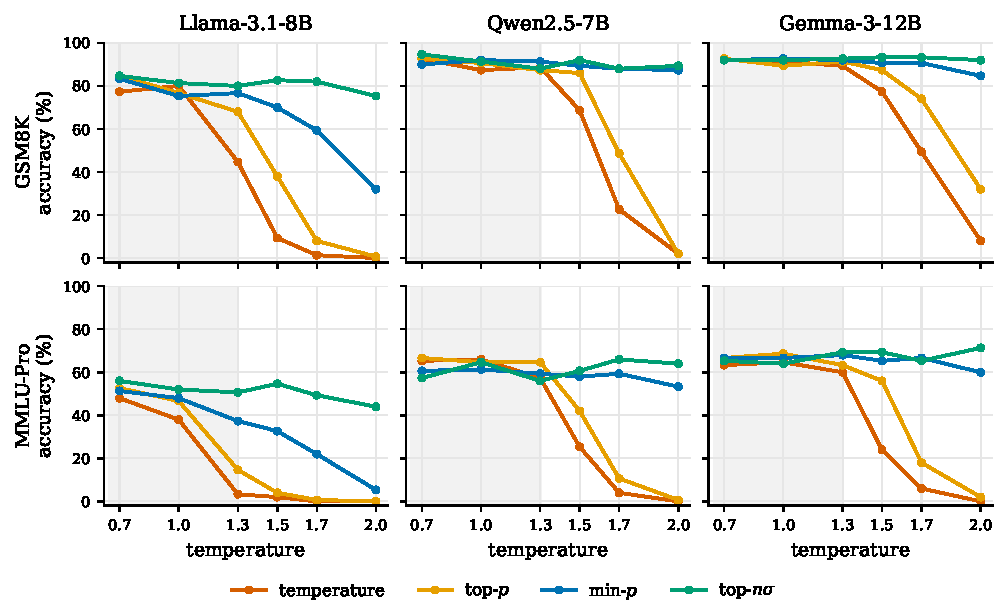
\includegraphics[width=0.78\textwidth]{fig3_cliff}
\caption{The cliff map. Accuracy versus temperature per sampler (the $T \le 1.0$ points
come from the main matrix; all at Q8). Each model has a cliff, and where it sits differs
by model. Truncation shifts each cliff right.}
\label{fig:cliff}
\end{figure*}

\begin{table}[t]
\centering
\caption{The cliff ladder: accuracy drop against each model's own $T{=}0.7$ anchor under
plain temperature (pp, 95\% item-clustered bootstrap CIs; Q8). The ladder is a separate
run from the main grid; its $T{=}1.3$ rung differs from Table~\ref{tab:collapse} by
amounts within the CIs (Appendix~\ref{app:repro}).}
\label{tab:cliff}
\footnotesize
\setlength{\tabcolsep}{2pt}
\begin{tabular}{lccc}
\toprule
$T$ & Llama-3.1-8B & Qwen2.5-7B & Gemma-3-12B \\
\midrule
\multicolumn{4}{l}{\emph{GSM8K}} \\
1.3 & $+32.7$ [24.7, 41.3] & $+4.0$ [$-0.7$, 9.3] & $+2.7$ [$-2.0$, 8.0] \\
1.5 & $+68.0$ [58.0, 76.7] & $+24.0$ [15.3, 33.3] & $+14.7$ [8.7, 21.3] \\
1.7 & $+76.0$ [66.7, 84.7] & $+70.0$ [62.0, 77.3] & $+42.7$ [34.7, 50.7] \\
2.0 & $+77.3$ [67.3, 86.0] & $+90.7$ [82.7, 97.3] & $+84.0$ [76.7, 90.7] \\
\midrule
\multicolumn{4}{l}{\emph{MMLU-Pro}} \\
1.3 & $+44.7$ [34.0, 56.0] & $+8.0$ [0.0, 16.7] & $+3.3$ [$-3.3$, 10.0] \\
1.5 & $+46.0$ [35.3, 57.3] & $+40.0$ [28.7, 52.0] & $+39.3$ [29.3, 48.7] \\
1.7 & $+48.0$ [36.7, 60.0] & $+61.3$ [48.7, 74.0] & $+57.3$ [45.3, 68.0] \\
2.0 & $+48.0$ [36.7, 59.3] & $+65.3$ [53.3, 78.0] & $+63.3$ [51.3, 75.3] \\
\bottomrule
\end{tabular}
\end{table}

\subsection{Quantization and answer agreement}
\label{sec:quant}

The results so far pool over the four quantization levels. For that to be safe,
quantization must not cost accuracy on its own, and it must not change what temperature
and the samplers do. Quantization costs little accuracy. From Q8\_0 down to Q3\_K\_M, greedy accuracy is
unchanged on every model of 7B parameters or more, and a real cost appears only on the
two smallest models, 7\,pp on Qwen3-4B and 9\,pp on Qwen3-1.7B. It changes nothing
about the collapse either. Recomputed separately at each level, the plain-temperature
drop of Section~\ref{sec:modelbound} shows Llama-3.1 collapsing at every level, with
drops of 30 to 47\,pp across levels and tasks, while no robust model exceeds 12\,pp at
any single level. Llama's sampler ordering at $T{=}1.3$ is identical at all four levels
(per-level values in Appendix~\ref{app:quant}).

A second check separates robustness from determinism. A model with very peaked
next-token distributions would also hold its accuracy, because sampling would return the
greedy path every time and the three repetitions of an item would come out as near
copies. The repetitions show the opposite. No item's three repetitions are identical on any model, yet the robust models still
converge on the answer, 1.1 to 1.4 distinct parsed answers per item on GSM8K at
$T{=}1.3$ (Mistral, whose low GSM8K accuracy scatters its answers, is 2.5;
Appendix~\ref{app:selfcons}). Llama-3.1 rises from 1.5 to 2.3 under the same
change, as each repetition derails on its own (full table in Appendix~\ref{app:selfcons}).
Neither quantization nor determinism explains the pattern.

\subsection{Toward a mechanism: per-token uncertainty predicts the ordering of drops}
\label{sec:mechanism}

If the collapse is a derailment process, fragile models should carry more per-token
uncertainty before any derailment happens. To measure that uncertainty we decode the
100 frozen prompts (the 50 items of each task) greedily on every model at Q8 and record
the raw top-20 next-token probabilities at each position. Each prompt is summarized by
four statistics of these distributions: an entropy lower bound (only the top 20
probabilities are observed), the top-1 probability and its margin over the top-2, and
the fraction of positions where the top-1 probability falls below 0.5. We decode greedily so that the statistics describe the text each model produces
when no random draw is involved, before any random draw can derail it.

Mean greedy-path entropy ranks the seven models' temperature drops at Spearman
$\rho = +0.93$ (flat-position fraction $+0.93$; top-1 margin $-0.93$; plotted in
Appendix~\ref{app:mechanism}). With seven models a rank correlation is fragile, so we report an item-clustered
bootstrap interval, $[+0.54, +0.96]$, and Appendix~\ref{app:mechanism} adds an exact
permutation test ($p = 0.007$) and leave-one-model-out ranges. The summaries cannot separate
one pair, though. Llama-3.1 and Mistral are nearly tied on every statistic we record,
0.33 versus 0.32 nats of entropy and $1.0 \times 10^{-3}$ probability mass beyond the
top 20 for both, yet Llama drops 40.8\,pp on MMLU-Pro and Mistral 8.0. Uncertainty on the greedy path predicts which models drop most, but not by how much.

The probe also estimates the per-token risk that drives a derailment. For each
position we compute the probability that sampling at $T{=}1.3$ picks a token from beyond
the model's own top 20; we call this the escape hazard (Appendix~\ref{app:mechanism} states the estimator and
its tail assumption). Llama's is 0.0033 per position
and Mistral's 0.0034, about 0.85 expected tail draws per 256 positions for both, and
across the seven models the hazard ranks the drops at the same $\rho = +0.93$ (bootstrap
$[+0.57, +0.96]$). Generation lengths show that a derailed generation does not recover: on every robust
model the length distribution of
finished generations is unchanged from $T{=}0.7$ to $T{=}1.3$ (90th-percentile ratio
0.85 to 1.19), and Llama's finished generations at $T{=}1.3$ are \emph{shorter}, because
only the short ones finish (Section~\ref{sec:degeneration}). Llama and Mistral therefore draw tail tokens equally often, and a generation that
derails does not come back, so what separates them must be how often a tail token starts
a derailment, that is, what happens after that token is in the context.

A perturbation experiment measures that directly. For each model and frozen prompt we
greedy-decode a 48-token prefix, replace the next token with the model's own rank-20
candidate at that position (median raw probability $2 \times 10^{-9}$, a genuine tail
draw), and continue greedily for 256 tokens, alongside a control continuation of the
unedited prefix. We then compare the two continuations' escape hazard over the 32 positions after
the injection.

Beyond the injected token itself, the continuations show no visible damage. They stay
coherent,
and Llama's reach the token cap no more often than its controls (14.0\% for both on
GSM8K). The difference is in the hazard. Llama's rises to 2.3 times its baseline
($+0.0042$ per position), Mistral's to 1.35 times ($+0.0012$), and no robust model gains more than $+0.0015$ (the absolute increase, not the ratio; Appendix~\ref{app:mechanism} explains why). This per-model increase ranks the temperature drops at
$\rho = +0.89$ (bootstrap $[+0.39, +0.96]$, permutation $p = 0.012$; the entropy
increase, $+0.86$).  With seven models these are consistency
checks, not a confirmed causal account. In short, Llama and Mistral draw tail tokens at the same rate, and what sets Llama
apart is how much one tail token raises the chance of the next.

\section{Discussion}
\label{sec:discussion}

\textbf{For practitioners.} At deployment temperatures the consequential choice is the
model: on a robust one every configuration we test stays within 10 points and most within 3,
on a fragile one the same sweep spans 42. Screening is cheap: fifty items under plain temperature at the top of the deployment
band suffice, and the drop in strict-parse rate between $T{=}0.7$ and 1.3 identifies a fragile model. In production, a derailed generation carries no well-formed answer, so simple output
validation catches it, while the rate of well-formed but wrong answers barely moves.

\textbf{For the sampler literature.} A sampler evaluation should say where its
models' cliffs sit, since a gain measured past one model's cliff need not exist on a
model whose cliff lies further out (Section~\ref{sec:cliff}).

\section{Conclusion}
Across nine models from five families, the choice of truncation sampler matters far less at deployment temperatures than the
model's own temperature sensitivity. Robust models hold within a few points
under every sampler we test, while two Llama generations lose up to 41 points under plain temperature and a third
loses 17 on the longer task. Each model we push past the deployment band collapses at its own temperature, Llama
already inside the band; truncation raises that temperature but changes little below it.
These results argue for screening temperature fragility before deployment rather than
tuning the sampler after it. What sets a model's cliff remains open.

\section*{Limitations}

Our sample is 50 items per task with $K{=}3$ repetitions per cell; the small item count
is what makes a factorial of 185{,}600 generations feasible. Item-clustered bootstrap CIs accompany every headline estimate, and the headline drops are 2 to 4 times their CI widths. Mistral-7B's GSM8K accuracy is low (32.7\% at $T{=}0.7$), which limits the power to
detect a further drop; its MMLU-Pro drop is measured away from floor and
its CI excludes zero. The frozen MMLU-Pro subset is single-category (business) because
the test split is sorted by category; the stratified $N{=}50$ replication of
Appendix~\ref{app:strat} reproduces the headline result.

The scope is open-weight instruction-tuned models of 1.7B to 12B parameters, served
through one inference engine. Whether larger or proprietary models share the Llama
family's fragility is untested. Both tasks are English, zero-shot, and objective: a
single exactly checkable answer is what lets the parser measure degeneration. The
original use case of truncation samplers, open-ended generation with no checkable
answer, lies outside this design, so our null result on sampler gains does not extend to
it. The recommendation to leave the sampler alone therefore applies to tasks with a
checkable answer, served through llama.cpp at the settings above; other engines, other quantization recipes, and open-ended generation are untested. All
Llama results come from imatrix GGUFs served by llama.cpp, with no full-precision or
second-engine Llama run, so a cause at the level of the conversion recipe or the engine,
common to all four quantization levels, is not excluded. Each truncation rule runs at one
setting, so the bound applies to those settings rather than to a tuned sampler, and the
sampler contrasts were not replicated on the stratified MMLU-Pro subset. Quantization covers llama.cpp k-quants only, one recipe by design so that the
quantization axis varies precision and nothing else; other recipes, and other engines'
sampler implementations, may behave differently. Thinking mode is off throughout the main grid; the thinking-on spot-check of
Appendix~\ref{app:thinking} agrees on GSM8K but shows a 10\,pp MMLU-Pro drop [2, 20] at
$N{=}25$, so our null does not cover thinking mode.

Every fragile model we observe is a Llama. The lineage run of
Section~\ref{sec:modelbound} shows the fragility spans three generations, which rules
out a quirk of one checkpoint. But the three releases share training data and
post-training methods, so they are not three independent pieces of evidence. With one
fragile family we cannot tell whether the fragility comes from a choice Llama made or
from something else these models have in common, and we cannot say how common such
families are.

Three analysis caveats. The max-minus-min sampler spread is biased upward, so it
overstates the differences between samplers; the bias is conservative for our claim that
those differences are small. Accuracy conditional on a strict parse is subject to survivorship bias, which
Section~\ref{sec:degeneration} estimates and corrects. The
mechanism probes correlate seven models, and Section~\ref{sec:mechanism} presents them
as consistency checks rather than a causal account. The bound of Section~\ref{sec:spread} is a pointwise 95\% upper limit on the sampler
effect at $N{=}50$ (7.8\,pp simultaneous), not
evidence of no effect, and the grid contains no base-versus-instruct or checkpoint axis,
so it can show that instruction tuning does not guarantee robustness but not what moves
the cliff. The forced-token experiment uses one configuration, a rank-20 token at
position 48 with a 32-position window, and we have not varied position, rank, or number
of injections. Mistral's GSM8K accuracy is low, so its comparison with Llama in
Section~\ref{sec:mechanism} rests on MMLU-Pro.

\bibliography{references}

\appendix

\section{Full sampler--temperature grids}
\label{app:grids}
Figure~\ref{fig:spread} plots the per-model sampler max$-$min spread of
Section~\ref{sec:spread} with its confidence intervals. Tables~\ref{tab:grid-gsm8k} and
\ref{tab:grid-mmlu} give the full main-matrix grids: accuracy for every sampler arm and
temperature, per model, pooled over quantization levels.
\begin{figure*}[t]
\centering
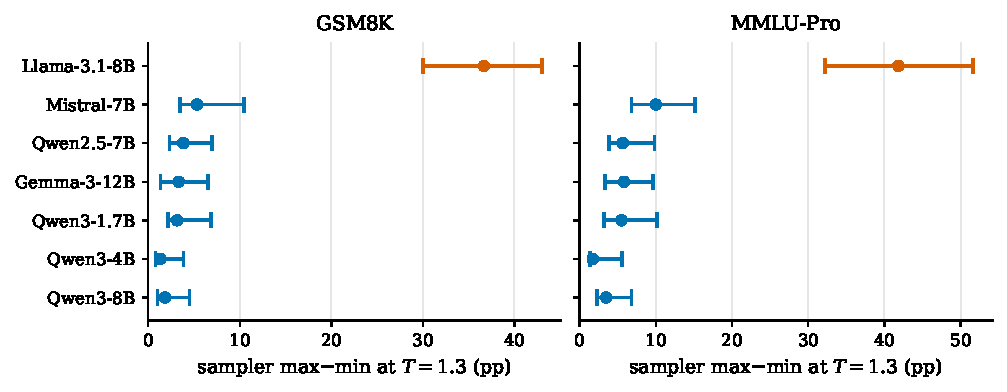
\includegraphics[width=0.9\textwidth]{fig4_spread}
\caption{Sampler max$-$min accuracy spread at $T{=}1.3$ per model (95\% CIs).}
\label{fig:spread}
\end{figure*}
\begin{table*}[p]\centering
\caption{GSM8K accuracy (\%) by sampler and temperature, pooled over quantization.}
\label{tab:grid-gsm8k}
\small\begin{tabular}{llccc}
\toprule
Model & Sampler & $T{=}0.7$ & $T{=}1.0$ & $T{=}1.3$ \\
\midrule
Llama-3.1-8B & greedy ($T{=}0$) & 78.0 & -- & -- \\
 & temperature & 78.2 & 74.8 & 44.2 \\
 & top-$k$ & 79.8 & 75.2 & 58.7 \\
 & top-$p$ & 81.5 & 78.0 & 63.8 \\
 & min-$p$ & 81.2 & 78.0 & 72.0 \\
 & top-$n\sigma$ & 78.8 & 80.7 & 80.8 \\
 & top-$p$ (temp-last) & 80.8 & 78.7 & 73.0 \\
 & min-$p$ (temp-last) & 78.7 & 81.3 & 76.2 \\
\midrule
Mistral-7B & greedy ($T{=}0$) & 31.0 & -- & -- \\
 & temperature & 32.7 & 30.0 & 29.2 \\
 & top-$k$ & 31.8 & 31.7 & 29.8 \\
 & top-$p$ & 28.2 & 31.0 & 34.2 \\
 & min-$p$ & 32.3 & 28.3 & 28.8 \\
 & top-$n\sigma$ & 29.5 & 30.7 & 30.2 \\
 & top-$p$ (temp-last) & 29.5 & 31.2 & 29.5 \\
 & min-$p$ (temp-last) & 29.5 & 32.0 & 30.5 \\
\midrule
Qwen2.5-7B & greedy ($T{=}0$) & 93.5 & -- & -- \\
 & temperature & 91.5 & 91.7 & 87.5 \\
 & top-$k$ & 90.2 & 88.5 & 88.7 \\
 & top-$p$ & 92.2 & 91.2 & 90.3 \\
 & min-$p$ & 90.8 & 90.5 & 91.0 \\
 & top-$n\sigma$ & 92.7 & 91.2 & 90.7 \\
 & top-$p$ (temp-last) & 90.8 & 91.3 & 90.3 \\
 & min-$p$ (temp-last) & 92.0 & 90.7 & 91.3 \\
\midrule
Gemma-3-12B & greedy ($T{=}0$) & 92.0 & -- & -- \\
 & temperature & 91.0 & 90.2 & 89.0 \\
 & top-$k$ & 91.8 & 91.7 & 90.7 \\
 & top-$p$ & 91.5 & 90.3 & 90.7 \\
 & min-$p$ & 91.5 & 91.3 & 92.3 \\
 & top-$n\sigma$ & 91.3 & 91.5 & 91.0 \\
 & top-$p$ (temp-last) & 90.2 & 91.8 & 91.5 \\
 & min-$p$ (temp-last) & 91.2 & 90.8 & 90.3 \\
\midrule
Qwen3-1.7B & greedy ($T{=}0$) & 75.5 & -- & -- \\
 & temperature & 73.3 & 73.7 & 73.7 \\
 & top-$k$ & 72.8 & 72.7 & 73.3 \\
 & top-$p$ & 73.8 & 75.0 & 72.7 \\
 & min-$p$ & 72.2 & 71.7 & 74.0 \\
 & top-$n\sigma$ & 74.3 & 73.5 & 72.3 \\
 & top-$p$ (temp-last) & 73.0 & 72.0 & 71.3 \\
 & min-$p$ (temp-last) & 74.7 & 73.3 & 74.5 \\
\midrule
Qwen3-4B & greedy ($T{=}0$) & 95.2 & -- & -- \\
 & temperature & 95.2 & 94.0 & 93.1 \\
 & top-$k$ & 94.0 & 94.5 & 94.1 \\
 & top-$p$ & 95.5 & 95.5 & 93.5 \\
 & min-$p$ & 95.1 & 94.7 & 92.9 \\
 & top-$n\sigma$ & 94.8 & 93.9 & 93.9 \\
 & top-$p$ (temp-last) & 94.8 & 95.2 & 94.3 \\
 & min-$p$ (temp-last) & 94.5 & 93.9 & 93.9 \\
\midrule
Qwen3-8B & greedy ($T{=}0$) & 94.5 & -- & -- \\
 & temperature & 95.0 & 94.2 & 94.5 \\
 & top-$k$ & 94.8 & 94.8 & 93.5 \\
 & top-$p$ & 94.0 & 94.3 & 93.7 \\
 & min-$p$ & 94.8 & 95.3 & 94.7 \\
 & top-$n\sigma$ & 96.3 & 94.2 & 94.3 \\
 & top-$p$ (temp-last) & 93.8 & 94.0 & 94.0 \\
 & min-$p$ (temp-last) & 96.2 & 94.7 & 95.3 \\
\bottomrule
\end{tabular}

\end{table*}
\begin{table*}[p]\centering
\caption{MMLU-Pro accuracy (\%) by sampler and temperature, pooled over quantization.}
\label{tab:grid-mmlu}
\small\begin{tabular}{llccc@{\hspace{14pt}}llccc}
\toprule
Model & Configuration & 0.7 & 1.0 & 1.3 & Model & Configuration & 0.7 & 1.0 & 1.3 \\
\midrule
Llama-3.1-8B & greedy & 54.0 & -- & -- & Qwen3-4B & greedy & 61.6 & -- & -- \\
 & temperature & 47.8 & 39.7 & 7.0 &  & temperature & 61.9 & 62.5 & 61.2 \\
 & top-$p$ & 51.3 & 46.0 & 16.0 &  & top-$p$ & 62.8 & 61.3 & 62.8 \\
 & top-$k$ & 51.2 & 43.3 & 26.8 &  & top-$k$ & 63.5 & 61.1 & 61.2 \\
 & min-$p$ & 51.2 & 50.8 & 39.5 &  & min-$p$ & 60.9 & 62.7 & 62.9 \\
 & top-$n\sigma$ & 51.0 & 50.5 & 48.8 &  & top-$n\sigma$ & 62.4 & 62.4 & 61.5 \\
 & top-$p$ (temp.\ last) & 50.3 & 46.7 & 37.5 &  & top-$p$ (temp.\ last) & 62.9 & 62.7 & 61.7 \\
 & min-$p$ (temp.\ last) & 51.2 & 50.2 & 43.5 &  & min-$p$ (temp.\ last) & 61.3 & 63.6 & 61.5 \\
\midrule
Mistral-7B & greedy & 35.5 & -- & -- & Qwen3-1.7B & greedy & 45.5 & -- & -- \\
 & temperature & 30.5 & 30.2 & 22.5 &  & temperature & 46.0 & 45.7 & 45.3 \\
 & top-$p$ & 30.2 & 29.5 & 25.3 &  & top-$p$ & 47.2 & 47.0 & 47.2 \\
 & top-$k$ & 32.5 & 32.3 & 28.3 &  & top-$k$ & 47.5 & 46.5 & 45.0 \\
 & min-$p$ & 33.8 & 30.7 & 31.0 &  & min-$p$ & 47.0 & 47.7 & 46.2 \\
 & top-$n\sigma$ & 32.3 & 31.5 & 31.5 &  & top-$n\sigma$ & 46.8 & 47.2 & 46.2 \\
 & top-$p$ (temp.\ last) & 29.2 & 30.2 & 32.5 &  & top-$p$ (temp.\ last) & 47.7 & 46.8 & 43.5 \\
 & min-$p$ (temp.\ last) & 33.2 & 33.3 & 28.7 &  & min-$p$ (temp.\ last) & 45.7 & 46.2 & 49.0 \\
\midrule
Qwen2.5-7B & greedy & 64.0 & -- & -- & Hermes-3-8B & greedy & 52.0 & -- & -- \\
 & temperature & 62.5 & 61.3 & 57.7 &  & temperature & 42.7 & 42.7 & 26.0 \\
 & top-$p$ & 65.5 & 62.8 & 62.7 &  & top-$p$ & 41.3 & 47.3 & 38.7 \\
 & top-$k$ & 62.5 & 61.7 & 57.0 &  & top-$k$ & 42.7 & 42.0 & 34.7 \\
 & min-$p$ & 61.3 & 63.5 & 59.7 &  & min-$p$ & 44.0 & 42.0 & 46.0 \\
 & top-$n\sigma$ & 62.0 & 63.5 & 61.0 &  & top-$n\sigma$ & 44.7 & 50.7 & 38.7 \\
 & top-$p$ (temp.\ last) & 63.7 & 62.7 & 61.3 &  & top-$p$ (temp.\ last) & 54.7 & 46.7 & 43.3 \\
 & min-$p$ (temp.\ last) & 64.2 & 63.0 & 62.3 &  & min-$p$ (temp.\ last) & 44.0 & 44.7 & 44.0 \\
\midrule
Gemma-3-12B & greedy & 61.0 & -- & -- & Qwen3.5-9B & greedy & 64.0 & -- & -- \\
 & temperature & 63.7 & 66.7 & 60.0 &  & temperature & 60.0 & 58.7 & 38.0 \\
 & top-$p$ & 65.7 & 66.7 & 63.8 &  & top-$p$ & 62.0 & 60.7 & 53.3 \\
 & top-$k$ & 64.3 & 62.8 & 63.7 &  & top-$k$ & 59.3 & 56.7 & 53.3 \\
 & min-$p$ & 65.3 & 67.0 & 65.5 &  & min-$p$ & 61.3 & 56.0 & 55.3 \\
 & top-$n\sigma$ & 65.2 & 65.8 & 65.8 &  & top-$n\sigma$ & 58.0 & 61.3 & 59.3 \\
 & top-$p$ (temp.\ last) & 65.8 & 65.0 & 65.2 &  & top-$p$ (temp.\ last) & 56.7 & 60.7 & 54.0 \\
 & min-$p$ (temp.\ last) & 65.3 & 63.7 & 63.8 &  & min-$p$ (temp.\ last) & 60.0 & 57.3 & 57.3 \\
\midrule
Qwen3-8B & greedy & 60.5 & -- & -- & OLMo-3-7B & greedy & 46.0 & -- & -- \\
 & temperature & 60.5 & 59.0 & 59.5 &  & temperature & 42.0 & 41.3 & 26.7 \\
 & top-$p$ & 60.5 & 61.3 & 60.5 &  & top-$p$ & 43.3 & 39.3 & 36.7 \\
 & top-$k$ & 60.2 & 61.3 & 57.0 &  & top-$k$ & 40.0 & 40.7 & 37.3 \\
 & min-$p$ & 61.0 & 59.2 & 59.7 &  & min-$p$ & 43.3 & 40.7 & 42.7 \\
 & top-$n\sigma$ & 60.0 & 58.8 & 58.7 &  & top-$n\sigma$ & 41.3 & 42.7 & 40.0 \\
 & top-$p$ (temp.\ last) & 60.7 & 59.5 & 60.5 &  & top-$p$ (temp.\ last) & 43.3 & 44.0 & 44.7 \\
 & min-$p$ (temp.\ last) & 61.3 & 60.7 & 59.3 &  & min-$p$ (temp.\ last) & 42.0 & 44.7 & 40.0 \\
\bottomrule
\end{tabular}

\end{table*}

\section{Degeneration decomposition}
\label{app:decomp}
Table~\ref{tab:decomp} decomposes accuracy under plain temperature sampling by parse path:
the strict final-answer-sentence rate, the parse-failure rate, the fraction of generations
that ran to the token cap (including outputs that llama.cpp returned through a parse error, which it raises on
degenerate text; the client recovers the text, and the record counts as at cap), and accuracy
conditional on a strict parse. Figure~\ref{fig:degenexamples} shows two representative
degenerate outputs.
Figure~\ref{fig:parsepaths} shows one generation per parse path. The
strict rule matches the pinned sentence with the answer directly after it, as in the
first example. The flexible rule catches two different things: a well-formed answer
written outside the pinned sentence, as in the second example, and a derailed generation
that still contains a number somewhere in its noise, which GSM8K then grades as a wrong
answer. Mistral omits the pinned sentence on 26 to 32\% of its GSM8K generations at every
temperature, and the Qwen3 models wrap the answer in markdown emphasis, which the strict
rule does not match; both grade correctly through the flexible rule. A failed parse is a
generation with no in-range letter or number at all. On MMLU-Pro that is almost always a
derailed generation, plus 13 to 16\% of Mistral's generations at every temperature that
name the option in words rather than by letter, and the markdown case of the third
example. Because markdown emphasis defeats the strict rule, we re-graded every record of
the main grid with a strict rule that tolerates it: 598 of 185,600 grades change, 556 of
them on Qwen3-8B and Qwen3-4B MMLU-Pro; no plain-temperature drop moves by more than
1.0\,pp and no deployment-band sampler spread by more than 2.0\,pp. The original parser, fixed before any run and mirroring lm-eval-harness, stays primary.

\begin{figure}[t]
\centering
\begin{minipage}{0.96\columnwidth}
\hrule\vspace{4pt}
{\small\ttfamily\raggedright
[strict] \ldots{} x = 19.50 / 0.75 \quad x = 26 \quad So the original price of the book
was \$26. \quad The final answer is \$26.
\par}
\vspace{4pt}\hrule\vspace{4pt}
{\small\ttfamily\raggedright
[flexible] \ldots{} 80 \textbackslash{}text\{ miles\} + 150 \textbackslash{}text\{ miles\}
= 230 \textbackslash{}text\{ miles\} \quad \#\#\# Final Answer: \quad The final answer is
\*\*230\*\*.
\par}
\vspace{4pt}\hrule\vspace{4pt}
{\small\ttfamily\raggedright
[failed] \ldots{} \textbackslash{}frac\{3,462.20\}\{35\} = 98.92 \quad \#\#\# Final
Answer: \quad The answer is \*\*J\*\*.
\par}
\vspace{4pt}\hrule
\end{minipage}
\caption{One generation per parse path (endings only). Strict: Llama-3.1-8B, GSM8K,
$T{=}1.3$, graded 26, correct. Flexible: Qwen3-8B, GSM8K, $T{=}0.7$; the emphasis
markers defeat the strict rule and the last-number fallback grades 230, correct. Failed:
Qwen3-8B, MMLU-Pro, $T{=}0.7$; no parenthesized letter anywhere, graded incorrect (the gold answer is E, so the incorrect grade is correct by coincidence).}
\label{fig:parsepaths}
\end{figure}
 The pattern is consistent: a coherent opening, a mid-generation
derailment, then token noise until the cap. The model never reaches an answer at all.

\begin{figure}[t]
\centering
\begin{minipage}{0.96\columnwidth}
\hrule\vspace{5pt}
{\small\ttfamily\raggedright
[opens] To solve this problem, we'll use the gross profit method of inventory
evaluation. Step 1: Calculate the gross profit earned during the year\ldots\\{}
[ends] H sieve Con Palette sediment conduit France called coaching OMAX may PHYS today
Enhanced vertices XOR/t and registration ordinances efforts yesterday Michael
\par}
\vspace{5pt}\hrule\vspace{5pt}
{\small\ttfamily\raggedright
[opens] To determine the correct type of research methods, we need to understand the
characteristics of each option: A. Non-probability: This method involves
selecting\ldots\\{}
[ends] entageeba lever modeling ign measures inherits cones quantum auditing\-ippines
image later campaigns Taylorart parte diesel El N resembled Dental professionals
\par}
\vspace{5pt}\hrule
\end{minipage}
\caption{Two representative degenerate outputs (Llama-3.1-8B, Q8, plain temperature,
$T{=}1.3$, MMLU-Pro; both ran to the 1024-token cap).}
\label{fig:degenexamples}
\end{figure}

Table~\ref{tab:recovery} gives the length-censoring evidence used in
Section~\ref{sec:mechanism}: run-to-cap rates and the 90th percentile of completion
length among \emph{terminated} generations at $T{=}0.7$ versus $T{=}1.3$. Robust models
are unchanged (ratio 0.85 to 1.19); Llama's surviving generations shorten ($\times$0.73
GSM8K, $\times$0.55 MMLU-Pro), so a derailed generation does not recover, and a generation survives only if it
finishes before its first bad draw.
\begin{table}[t]\centering
\caption{Terminated-length censoring under plain temperature at $T{=}0.7$ versus
$T{=}1.3$ (pooled over quantization). ``At cap'' includes parse-error-recovered outputs (Appendix~\ref{app:decomp}).}
\label{tab:recovery}
\small\setlength{\tabcolsep}{2.2pt}\begin{tabular}{llccccc}
\toprule
 & & \multicolumn{2}{c}{at cap (\%)} & \multicolumn{2}{c}{p90 length} & \\
Model & Task & $T{=}0.7$ & $T{=}1.3$ & $T{=}0.7$ & $T{=}1.3$ & ratio \\
\midrule
Llama-3.1-8B & GSM8K & 5.2 & 53.8 & 318 & 232 & 0.73$\times$ \\
 & MMLU-Pro & 11.0 & 89.2 & 633 & 345 & 0.55$\times$ \\
\midrule
Mistral-7B & GSM8K & 3.5 & 8.3 & 367 & 378 & 1.03$\times$ \\
 & MMLU-Pro & 1.0 & 12.5 & 628 & 750 & 1.19$\times$ \\
\midrule
Qwen2.5-7B & GSM8K & 0.2 & 1.7 & 341 & 361 & 1.06$\times$ \\
 & MMLU-Pro & 2.5 & 10.2 & 771 & 732 & 0.95$\times$ \\
\midrule
Gemma-3-12B & GSM8K & 2.0 & 5.3 & 363 & 344 & 0.95$\times$ \\
 & MMLU-Pro & 9.8 & 17.2 & 753 & 763 & 1.01$\times$ \\
\midrule
Qwen3-1.7B & GSM8K & 2.0 & 2.2 & 324 & 339 & 1.05$\times$ \\
 & MMLU-Pro & 15.8 & 16.3 & 779 & 806 & 1.03$\times$ \\
\midrule
Qwen3-4B & GSM8K & 0.9 & 0.8 & 353 & 361 & 1.02$\times$ \\
 & MMLU-Pro & 11.9 & 12.4 & 778 & 731 & 0.94$\times$ \\
\midrule
Qwen3-8B & GSM8K & 2.3 & 2.3 & 379 & 389 & 1.03$\times$ \\
 & MMLU-Pro & 12.3 & 16.0 & 850 & 724 & 0.85$\times$ \\
\bottomrule
\end{tabular}

\end{table}
\begin{table*}[t]\centering
\caption{Decomposition of the temperature effect (plain temperature, pooled over
quantization; \%).}
\label{tab:decomp}
\small\begin{tabular}{llcccccc}
\toprule
Model & Task & $T$ & acc & strict & failed & at cap & acc$|$strict \\
\midrule
Llama-3.1-8B & GSM8K & 0.7 & 78.2 & 93.0 & 0.0 & 5.2 & 83.0 \\
 & GSM8K & 1.0 & 74.8 & 84.7 & 0.0 & 7.8 & 86.4 \\
 & GSM8K & 1.3 & 44.2 & 43.8 & 0.5 & 53.8 & 97.3 \\
 & MMLU-Pro & 0.7 & 47.8 & 82.3 & 15.3 & 11.0 & 58.1 \\
 & MMLU-Pro & 1.0 & 39.7 & 64.8 & 29.0 & 23.7 & 60.2 \\
 & MMLU-Pro & 1.3 & 7.0 & 8.7 & 84.5 & 89.2 & 76.9 \\
\midrule
Mistral-7B & GSM8K & 0.7 & 32.7 & 72.2 & 0.3 & 3.5 & 34.2 \\
 & GSM8K & 1.0 & 30.0 & 67.7 & 0.0 & 4.3 & 32.8 \\
 & GSM8K & 1.3 & 29.2 & 62.8 & 0.0 & 8.3 & 29.2 \\
 & MMLU-Pro & 0.7 & 30.5 & 84.0 & 12.8 & 1.0 & 35.7 \\
 & MMLU-Pro & 1.0 & 30.2 & 80.8 & 17.0 & 1.0 & 37.1 \\
 & MMLU-Pro & 1.3 & 22.5 & 73.5 & 21.2 & 12.5 & 29.9 \\
\midrule
Qwen2.5-7B & GSM8K & 0.7 & 91.5 & 98.3 & 0.0 & 0.2 & 92.5 \\
 & GSM8K & 1.0 & 91.7 & 95.7 & 0.0 & 0.5 & 92.7 \\
 & GSM8K & 1.3 & 87.5 & 92.5 & 0.0 & 1.7 & 90.1 \\
 & MMLU-Pro & 0.7 & 62.5 & 97.3 & 2.3 & 2.5 & 64.2 \\
 & MMLU-Pro & 1.0 & 61.3 & 96.5 & 2.5 & 3.0 & 63.4 \\
 & MMLU-Pro & 1.3 & 57.7 & 87.3 & 10.5 & 10.2 & 65.6 \\
\midrule
Gemma-3-12B & GSM8K & 0.7 & 91.0 & 98.0 & 0.0 & 2.0 & 92.3 \\
 & GSM8K & 1.0 & 90.2 & 96.8 & 0.0 & 3.3 & 93.1 \\
 & GSM8K & 1.3 & 89.0 & 94.5 & 0.0 & 5.3 & 93.8 \\
 & MMLU-Pro & 0.7 & 63.7 & 90.3 & 9.0 & 9.8 & 70.5 \\
 & MMLU-Pro & 1.0 & 66.7 & 89.7 & 8.2 & 10.3 & 74.3 \\
 & MMLU-Pro & 1.3 & 60.0 & 82.8 & 14.5 & 17.2 & 72.2 \\
\midrule
Qwen3-1.7B & GSM8K & 0.7 & 73.3 & 20.3 & 0.0 & 2.0 & 73.8 \\
 & GSM8K & 1.0 & 73.7 & 20.0 & 0.0 & 0.7 & 71.7 \\
 & GSM8K & 1.3 & 73.7 & 19.0 & 0.0 & 2.2 & 71.1 \\
 & MMLU-Pro & 0.7 & 46.0 & 83.7 & 13.3 & 15.8 & 54.8 \\
 & MMLU-Pro & 1.0 & 45.7 & 82.2 & 15.5 & 16.3 & 55.4 \\
 & MMLU-Pro & 1.3 & 45.3 & 83.2 & 13.5 & 16.3 & 54.5 \\
\midrule
Qwen3-4B & GSM8K & 0.7 & 95.2 & 94.3 & 0.0 & 0.9 & 95.3 \\
 & GSM8K & 1.0 & 94.0 & 92.3 & 0.0 & 0.8 & 94.8 \\
 & GSM8K & 1.3 & 93.1 & 95.6 & 0.0 & 0.8 & 93.7 \\
 & MMLU-Pro & 0.7 & 61.9 & 87.2 & 12.5 & 11.9 & 70.9 \\
 & MMLU-Pro & 1.0 & 62.5 & 87.3 & 12.0 & 10.8 & 71.6 \\
 & MMLU-Pro & 1.3 & 61.2 & 87.5 & 11.1 & 12.4 & 70.0 \\
\midrule
Qwen3-8B & GSM8K & 0.7 & 95.0 & 48.2 & 0.0 & 2.3 & 98.3 \\
 & GSM8K & 1.0 & 94.2 & 49.2 & 0.0 & 2.3 & 98.6 \\
 & GSM8K & 1.3 & 94.5 & 52.2 & 0.0 & 2.3 & 98.1 \\
 & MMLU-Pro & 0.7 & 60.5 & 82.5 & 15.2 & 12.3 & 72.3 \\
 & MMLU-Pro & 1.0 & 59.0 & 80.5 & 15.5 & 14.8 & 72.3 \\
 & MMLU-Pro & 1.3 & 59.5 & 79.8 & 16.3 & 16.0 & 73.5 \\
\bottomrule
\end{tabular}

\end{table*}

\section{Stratified MMLU-Pro replication}
\label{app:strat}
The frozen $N{=}50$ MMLU-Pro head subset is single-category (business) because the test
split is sorted by category. Table~\ref{tab:strat} repeats the pure-temperature axis (Q8,
$K{=}3$) on a deterministic stratified subset with 3--4 items from each of the 14
categories. The collapse ordering reproduces.
\begin{table}[t]\centering
\caption{Stratified versus head-of-split (business) MMLU-Pro subset; plain temperature
accuracy (\%) at Q8\_0.}
\label{tab:strat}
\small\setlength{\tabcolsep}{3pt}\begin{tabular}{llcccc}
\toprule
Model & Subset & $T{=}0.7$ & $T{=}1.0$ & $T{=}1.3$ & drop \\
\midrule
Llama-3.1-8B & stratified & 44.7 & 38.7 & 1.3 & $+43.3$\,pp \\
Llama-3.1-8B & business (head-50) & 48.0 & 38.0 & 10.0 & $+38.0$\,pp \\
\midrule
Qwen2.5-7B & stratified & 54.7 & 53.3 & 48.7 & $+6.0$\,pp \\
Qwen2.5-7B & business (head-50) & 65.3 & 66.0 & 58.0 & $+7.3$\,pp \\
\midrule
Gemma-3-12B & stratified & 64.0 & 62.7 & 56.7 & $+7.3$\,pp \\
Gemma-3-12B & business (head-50) & 63.3 & 64.7 & 60.0 & $+3.3$\,pp \\
\bottomrule
\end{tabular}

\end{table}

\section{Llama lineage run}
\label{app:lineage}
The lineage run repeats the pure-temperature axis (greedy anchor plus plain temperature
at $T \in \{0.7, 1.0, 1.3\}$) on Llama-3-8B and Llama-3.2-3B: Q8\_0, both frozen
$N{=}50$ tasks, $K{=}3$, 2{,}000 generations, same pipeline, prompts, and seed
derivation as the main matrix. Table~\ref{tab:lineage} reports both models next to the
Q8-only Llama-3.1-8B slice of the main matrix, which is why the Llama-3.1 numbers differ
slightly from the quantization-pooled Table~\ref{tab:collapse}. Greedy anchors are
ordinary (Llama-3-8B 76.0\% GSM8K / 40.0\% MMLU-Pro; Llama-3.2-3B 74.0 / 42.0\%).
Llama-3.2-3B reproduces the full degeneration signature at $T{=}1.3$: strict-parse rate
98.7 $\to$ 41.3\% on GSM8K and 82.7 $\to$ 6.0\% on MMLU-Pro, 50 to 51\% of generations
at the token cap, and accuracy conditional on a strict parse at or above the greedy
level (85.5 and 55.6\%). Llama-3-8B's MMLU-Pro drop has a milder surface: strict-parse
97.3 $\to$ 65.3\% with only 4.7\% at the cap, so its lost generations mostly terminate
as parse failures short of the cap.
\begin{table}[t]\centering
\caption{Llama lineage: plain-temperature accuracy and $T0.7 \to 1.3$ drop (pp, 95\%
item-clustered bootstrap CIs), all at Q8\_0. The Llama-3.1-8B rows are the Q8-only slice
of the main matrix.}
\label{tab:lineage}
\small\setlength{\tabcolsep}{1.6pt}\begin{tabular}{llccc}
\toprule
 & & \multicolumn{2}{c}{acc (\%) at $T$} & \\
Model & Task & 0.7 & 1.3 & drop [95\% CI] \\
\midrule
Llama-3-8B & GSM8K & 75.3 & 71.3 & $+4.0$\,[$-2.7$,\,11.3] \\
 & MMLU-Pro & 44.0 & 27.3 & $+16.7$\,[9.3,\,24.0] \\
\midrule
Llama-3.1-8B & GSM8K & 77.3 & 47.3 & $+30.0$\,[21.3,\,38.7] \\
 & MMLU-Pro & 48.0 & 10.0 & $+38.0$\,[28.0,\,48.7] \\
\midrule
Llama-3.2-3B & GSM8K & 74.0 & 36.0 & $+38.0$\,[29.3,\,47.3] \\
 & MMLU-Pro & 40.0 & 3.3 & $+36.7$\,[26.7,\,46.0] \\
\bottomrule
\end{tabular}

\end{table}

\section{High-temperature regime}
\label{app:hight}
Table~\ref{tab:hightemp} reports a small probe ($N{=}15$, $K{=}3$, Q8) in the regime
where min-$p$ and top-$n\sigma$ report their largest gains. The sampler ordering is
top-$n\sigma$ $\gg$ min-$p$ $\gg$ top-$p$ $\approx$ temperature; every generation in the zero cells ran to the token cap, and even the most robust model collapses under plain
temperature.
\begin{table}[t]\centering
\caption{Accuracy (\%) at $T{=}2$ and $T{=}3$ (45 observations per cell).}
\label{tab:hightemp}
\small\setlength{\tabcolsep}{3pt}\begin{tabular}{llcccc}
\toprule
 & & \multicolumn{2}{c}{Llama-3.1-8B} & \multicolumn{2}{c}{Gemma-3-12B} \\
Task & Sampler & $T{=}2$ & $T{=}3$ & $T{=}2$ & $T{=}3$ \\
\midrule
GSM8K & temperature & 0 & 0 & 16 & 0 \\
 & top-$p$ & 0 & 0 & 27 & 0 \\
 & min-$p$ & 33 & 0 & 78 & 24 \\
 & top-$n\sigma$ & 71 & 80 & 87 & 89 \\
\midrule
MMLU-Pro & temperature & 0 & 0 & 0 & 0 \\
 & top-$p$ & 0 & 0 & 0 & 0 \\
 & min-$p$ & 0 & 0 & 58 & 0 \\
 & top-$n\sigma$ & 47 & 51 & 69 & 62 \\
\bottomrule
\end{tabular}

\end{table}

\section{Temperature-first versus temperature-last}
\label{app:tlast}
Table~\ref{tab:tlast} gives both chain orders for the two probability-space truncators.
The two orders are indistinguishable on the robust models. On Llama at $T{=}1.3$,
truncating before temperature scaling is more protective, worth $+9.2$\,pp on GSM8K and
$+21.5$\,pp on MMLU-Pro for top-$p$ ($+4.2$ and $+4.0$ for min-$p$); the results section
explains why.
\begin{table*}[t]\centering
\caption{Accuracy (\%) with temperature applied before (left) versus after (right)
truncation, pooled over quantization.}
\label{tab:tlast}
\small\begin{tabular}{llcccccc}
\toprule
 & & \multicolumn{3}{c}{temperature-first} & \multicolumn{3}{c}{temperature-last} \\
Model & Method & 0.7 & 1.0 & 1.3 & 0.7 & 1.0 & 1.3 \\
\midrule
\multicolumn{8}{l}{\emph{GSM8K}} \\
Llama-3.1-8B & top-$p$ & 81.5 & 78.0 & 63.8 & 80.8 & 78.7 & 73.0 \\
Llama-3.1-8B & min-$p$ & 81.2 & 78.0 & 72.0 & 78.7 & 81.3 & 76.2 \\
Mistral-7B & top-$p$ & 28.2 & 31.0 & 34.2 & 29.5 & 31.2 & 29.5 \\
Mistral-7B & min-$p$ & 32.3 & 28.3 & 28.8 & 29.5 & 32.0 & 30.5 \\
Qwen2.5-7B & top-$p$ & 92.2 & 91.2 & 90.3 & 90.8 & 91.3 & 90.3 \\
Qwen2.5-7B & min-$p$ & 90.8 & 90.5 & 91.0 & 92.0 & 90.7 & 91.3 \\
Gemma-3-12B & top-$p$ & 91.5 & 90.3 & 90.7 & 90.2 & 91.8 & 91.5 \\
Gemma-3-12B & min-$p$ & 91.5 & 91.3 & 92.3 & 91.2 & 90.8 & 90.3 \\
Qwen3-1.7B & top-$p$ & 73.8 & 75.0 & 72.7 & 73.0 & 72.0 & 71.3 \\
Qwen3-1.7B & min-$p$ & 72.2 & 71.7 & 74.0 & 74.7 & 73.3 & 74.5 \\
Qwen3-4B & top-$p$ & 95.5 & 95.5 & 93.5 & 94.8 & 95.2 & 94.3 \\
Qwen3-4B & min-$p$ & 95.1 & 94.7 & 92.9 & 94.5 & 93.9 & 93.9 \\
Qwen3-8B & top-$p$ & 94.0 & 94.3 & 93.7 & 93.8 & 94.0 & 94.0 \\
Qwen3-8B & min-$p$ & 94.8 & 95.3 & 94.7 & 96.2 & 94.7 & 95.3 \\
\midrule
\multicolumn{8}{l}{\emph{MMLU-Pro}} \\
Llama-3.1-8B & top-$p$ & 51.3 & 46.0 & 16.0 & 50.3 & 46.7 & 37.5 \\
Llama-3.1-8B & min-$p$ & 51.2 & 50.8 & 39.5 & 51.2 & 50.2 & 43.5 \\
Mistral-7B & top-$p$ & 30.2 & 29.5 & 25.3 & 29.2 & 30.2 & 32.5 \\
Mistral-7B & min-$p$ & 33.8 & 30.7 & 31.0 & 33.2 & 33.3 & 28.7 \\
Qwen2.5-7B & top-$p$ & 65.5 & 62.8 & 62.7 & 63.7 & 62.7 & 61.3 \\
Qwen2.5-7B & min-$p$ & 61.3 & 63.5 & 59.7 & 64.2 & 63.0 & 62.3 \\
Gemma-3-12B & top-$p$ & 65.7 & 66.7 & 63.8 & 65.8 & 65.0 & 65.2 \\
Gemma-3-12B & min-$p$ & 65.3 & 67.0 & 65.5 & 65.3 & 63.7 & 63.8 \\
Qwen3-1.7B & top-$p$ & 47.2 & 47.0 & 47.2 & 47.7 & 46.8 & 43.5 \\
Qwen3-1.7B & min-$p$ & 47.0 & 47.7 & 46.2 & 45.7 & 46.2 & 49.0 \\
Qwen3-4B & top-$p$ & 62.8 & 61.3 & 62.8 & 62.9 & 62.7 & 61.7 \\
Qwen3-4B & min-$p$ & 60.9 & 62.7 & 62.9 & 61.3 & 63.6 & 61.5 \\
Qwen3-8B & top-$p$ & 60.5 & 61.3 & 60.5 & 60.7 & 59.5 & 60.5 \\
Qwen3-8B & min-$p$ & 61.0 & 59.2 & 59.7 & 61.3 & 60.7 & 59.3 \\
\bottomrule
\end{tabular}

\end{table*}

\section{Thinking-mode spot-check}
\label{app:thinking}
The matrix runs Qwen3 with thinking off. A confirmatory spot-check (Qwen3-8B, Q8,
thinking on, 450 generations, $N{=}25$, $K{=}2$) reproduces the GSM8K result (94\% at $T{=}0.7$ versus 96\% at $T{=}1.3$ under plain
temperature) but not the MMLU-Pro one: 56\% versus 46\%, a 10\,pp drop with
item-clustered CI [2, 20] at $N{=}25$, with min-$p$ flat on both tasks. With thinking
on, the longer traces make Qwen3-8B less robust on the longer task, so the thinking-off
null of the main grid should not be read as covering thinking mode.

\section{Per-quantization-level temperature drops}
\label{app:quant}
Figure~\ref{fig:quant} plots the direct cost of quantization on greedy accuracy.
Table~\ref{tab:quantdrop} recomputes the plain-temperature drop of
Table~\ref{tab:collapse} separately at each quantization level. Each cell pools 150
generations ($N{=}50$, $K{=}3$), so single-level estimates are noisier than the pooled
ones. The BF16 anchor on Qwen3-4B shows the same null drop as its quantized versions
($-1.3$\,pp GSM8K, $-2.0$\,pp MMLU-Pro).
\begin{figure}[t]
\centering
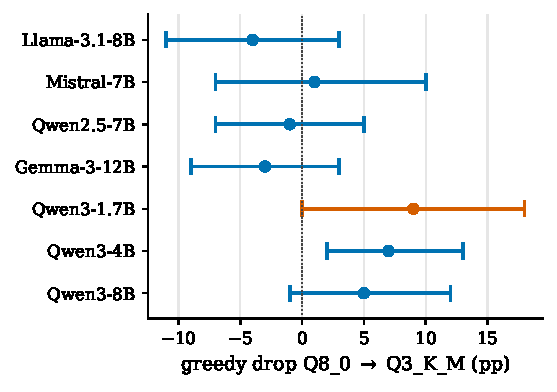
\includegraphics[width=\linewidth]{fig5_quant}
\caption{Greedy accuracy drop Q8\_0 $\to$ Q3\_K\_M per model (95\% CIs), pooled tasks.}
\label{fig:quant}
\end{figure}
\begin{table}[h]\centering
\caption{Plain-temperature accuracy drop $T0.7 \to 1.3$ (pp) per quantization level.}
\label{tab:quantdrop}
\small\begin{tabular}{lcccc}
\toprule
Model & Q8\_0 & Q6\_K & Q4\_K\_M & Q3\_K\_M \\
\midrule
\multicolumn{5}{l}{\emph{GSM8K}} \\
Llama-3.1-8B & $+30.0$ & $+32.0$ & $+36.0$ & $+38.0$ \\
Mistral-7B & $-0.7$ & $-0.7$ & $+3.3$ & $+12.0$ \\
Qwen2.5-7B & $+4.0$ & $+2.7$ & $+2.7$ & $+6.7$ \\
Gemma-3-12B & $+3.3$ & $+2.7$ & $+0.0$ & $+2.0$ \\
Qwen3-1.7B & $+5.3$ & $-6.0$ & $-0.7$ & $+0.0$ \\
Qwen3-4B & $+2.7$ & $+0.7$ & $+6.0$ & $+2.7$ \\
Qwen3-8B & $-2.0$ & $+1.3$ & $+2.0$ & $+0.7$ \\
\midrule
\multicolumn{5}{l}{\emph{MMLU-Pro}} \\
Llama-3.1-8B & $+38.0$ & $+46.7$ & $+38.0$ & $+40.7$ \\
Mistral-7B & $+9.3$ & $+5.3$ & $+10.7$ & $+6.7$ \\
Qwen2.5-7B & $+7.3$ & $+6.0$ & $+4.0$ & $+2.0$ \\
Gemma-3-12B & $+3.3$ & $+5.3$ & $+2.7$ & $+3.3$ \\
Qwen3-1.7B & $+0.7$ & $+6.0$ & $-8.0$ & $+4.0$ \\
Qwen3-4B & $-0.7$ & $+0.0$ & $+2.0$ & $+4.0$ \\
Qwen3-8B & $+2.7$ & $-0.7$ & $+0.0$ & $+2.0$ \\
\bottomrule
\end{tabular}

\end{table}

\section{Answer agreement across repetitions}
\label{app:selfcons}
Mean distinct parsed answers per item across the $K{=}3$ repetitions under plain
temperature (Table~\ref{tab:selfcons}). Robust models sample diverse token sequences that
converge on the same answer; a parse failure counts as one distinct answer, so the
statistic is a divergence proxy; it is the per-item agreement that self-consistency
decoding \citep{wang2023selfconsistency} exploits by majority vote. The parse-failure
convention censors Llama-3.1 on
MMLU-Pro at $T{=}1.3$: with 84.5\% of generations failing to parse, the repetitions
agree on having no answer, and the statistic falls to 1.28. Mistral sits near 2.2
distinct answers at both temperatures, and its scatter has a different source: at a
greedy GSM8K accuracy of 31\%, most repetitions are wrong, and wrong repetitions rarely
agree on the same wrong number at any temperature. The shift attributable to
temperature is $+0.27$.
\begin{table}[h]\centering
\caption{Mean distinct parsed answers per item ($K{=}3$, pooled over quantization).}
\label{tab:selfcons}
\small\begin{tabular}{lcccc}
\toprule
 & \multicolumn{2}{c}{GSM8K} & \multicolumn{2}{c}{MMLU-Pro} \\
Model & $T{=}0.7$ & $T{=}1.3$ & $T{=}0.7$ & $T{=}1.3$ \\
\midrule
Llama-3.1-8B & 1.51 & 2.33 & 1.71 & 1.28 \\
Mistral-7B & 2.21 & 2.48 & 1.97 & 2.21 \\
Qwen2.5-7B & 1.10 & 1.27 & 1.44 & 1.57 \\
Gemma-3-12B & 1.12 & 1.16 & 1.33 & 1.45 \\
Qwen3-1.7B & 1.41 & 1.43 & 1.67 & 1.73 \\
Qwen3-4B & 1.05 & 1.14 & 1.33 & 1.38 \\
Qwen3-8B & 1.09 & 1.13 & 1.41 & 1.40 \\
\bottomrule
\end{tabular}

\end{table}

\section{Mechanism probes}
\label{app:mechanism}
Figure~\ref{fig:mechanism} plots greedy-path entropy against the temperature drop.
Table~\ref{tab:mechanism} consolidates the per-model mechanism evidence of
Section~\ref{sec:mechanism}: greedy-path entropy lower bound and flat-position fraction
(top-1 $<$ 0.5) from the summary probe; the temperature-scaled beyond-top-20 escape
hazard per position at $T{=}1.3$ from the raw top-20 arrays; and the perturbation
deltas (post-injection minus control over 32 positions, escape hazard and entropy) from
the forced-token experiment. Escape columns are $\times 10^{-3}$. The escape hazard at temperature $T$ is computed
from the raw top-20 probabilities $p_1 \ge \dots \ge p_{20}$ and the residual mass
$t = 1 - \sum_i p_i$ as $S_\text{tail}/(S_\text{top} + S_\text{tail})$ with
$S_\text{top} = \sum_i p_i^{1/T}$; the scaled tail mass is not identifiable from the top
20, so we assume the tail consists of $t/p_{20}$ tokens of probability $p_{20}$,
$S_\text{tail} = (t/p_{20})\,p_{20}^{1/T}$. The one-token lower bound
$S_\text{tail} = t^{1/T}$ ranks the models identically ($\rho = +0.93$). Leaving out any
one model, $\rho$ ranges over $[+0.89, +0.94]$ for entropy and for the hazard, and over
$[+0.83, +1.00]$ for the perturbation response. Every static column ties Llama-3.1 with Mistral; only the perturbation response separates
them. We use the absolute post-injection hazard increase because survival over $L$ tokens
scales as $(1-h)^L$ in the absolute hazard $h$; it ranks the drops at $\rho = +0.89$,
while the ratio of injected to control hazard does not ($\rho = +0.11$), because Gemma-3
and Qwen3-4B triple a hazard that starts far below Llama's baseline.
\begin{figure}[t]
\centering
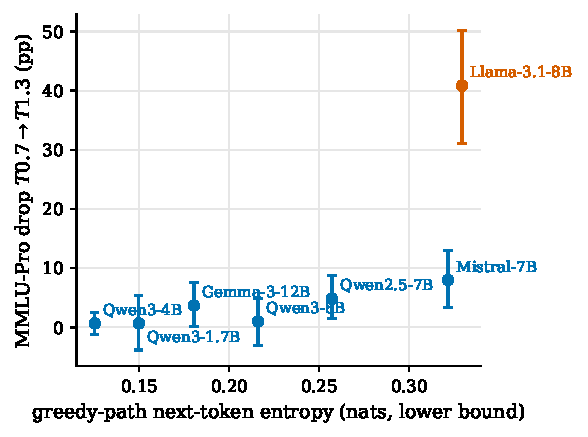
\includegraphics[width=\linewidth]{fig6_mechanism}
\caption{Per-token uncertainty on the model's own greedy path versus the temperature
drop (MMLU-Pro, 95\% CIs). The rank correlation is $\rho = +0.93$; the Llama--Mistral gap
at equal entropy shows flatness alone does not set the magnitude.}
\label{fig:mechanism}
\end{figure}
\begin{table}[t]\centering
\caption{Mechanism probes per model (Q8, 100 frozen prompts). Escape hazards are at
$T{=}1.3$; drop is the MMLU-Pro plain-temperature $T0.7 \to 1.3$ accuracy drop (pp),
pooled over quantization.}
\label{tab:mechanism}
\small\setlength{\tabcolsep}{3pt}\begin{tabular}{lcccccc}
\toprule
Model & $H_{lb}$ & flat\% & esc & $\Delta$esc & $\Delta H$ & drop \\
\midrule
Llama-3.1-8B & 0.329 & 7.1 & 3.26 & +4.20 & +0.110 & +40.8 \\
Mistral-7B & 0.322 & 6.8 & 3.40 & +1.19 & +0.044 & +8.0 \\
Qwen2.5-7B & 0.257 & 4.8 & 1.97 & +1.00 & +0.049 & +4.8 \\
Gemma-3-12B & 0.180 & 3.0 & 1.44 & +1.42 & +0.055 & +3.7 \\
Qwen3-1.7B & 0.150 & 2.1 & 0.36 & -0.00 & +0.012 & +0.7 \\
Qwen3-4B & 0.125 & 1.5 & 0.22 & +0.21 & +0.021 & +0.7 \\
Qwen3-8B & 0.216 & 3.8 & 0.71 & +0.22 & +0.024 & +1.0 \\
\bottomrule
\end{tabular}

\end{table}

\section{Bound on the sampler effect}
\label{app:bound}
Table~\ref{tab:bound} gives every paired contrast behind Section~\ref{sec:spread}: for each model, task, and
temperature, the accuracy of each of the six truncation arms minus plain
temperature on the same 50 items (each item's accuracy is its mean over $K{=}3$
repetitions and the quantization levels, five for Qwen3-4B), with a 95\% item-clustered bootstrap CI
($B{=}5000$). Entries whose interval lies above zero are in bold. A generalized estimating
equation over the same records, with an identity link, item clusters, and an
exchangeable working correlation, gives the same point estimates and intervals that
differ by at most 0.6\,pp (median 0.1); scripts \texttt{sampler\_bound.py} and
\texttt{sampler\_gee.py}.
\begin{table*}[t]\centering
\caption{Paired accuracy difference of each truncation arm against plain temperature
(pp, 95\% item-clustered bootstrap CIs; pooled over quantization). Bold: interval above
zero.}
\label{tab:bound}
\footnotesize\setlength{\tabcolsep}{4pt}\resizebox{\textwidth}{!}{\begin{tabular}{llrrrr}
\toprule
Models & $T$ & comparisons & largest gain (pp) & upper bound (pp) & intervals above 0 \\
\midrule
six robust models, all quantization levels & 0.7, 1.0 & 96 & $+3.3$ & 9.0 & 1 \\
six robust models, Q8\_0 only & 0.7, 1.0 & 96 & $+4.7$ & 16.0 & 0 \\
six robust models, all quantization levels & 1.3 & 48 & $+9.0$ & -- & 13 \\
Llama-3.1-8B, all quantization levels & 0.7, 1.0 & 16 & $+11.2$ & 16.8 & 6 \\
three flagged models, Q8\_0 & 0.7, 1.0 & 48 & $+8.0$ & 18.0 & 2 \\
three flagged models, Q8\_0 & 1.3 & 24 & $+21.3$ & 32.7 & 20 \\
\bottomrule
\end{tabular}
}
\end{table*}

\section{Reproducibility}
\label{app:repro}
\begin{itemize}
  \item \textbf{Inference stack.} llama.cpp at commit \texttt{5aba5364} (server build
    9456), native \texttt{/completion} endpoint, CUDA builds of the same commit per GPU
    architecture (sm\_75 for RTX 2080~Ti, sm\_120 for RTX 5070~Ti). Server-side BOS
    insertion is disabled; the client-rendered chat template owns the special tokens, and
    each record stores the SHA-256 of the exact rendered prompt.
  \item \textbf{Quantizations.} Every quantized checkpoint is a Bartowski imatrix GGUF
    (one provider, one recipe, so the quantization axis is not confounded by recipe).
    SHA-256 hashes of all 31 model files are pinned in the repository
    (\texttt{DOWNLOADS.md}).
  \item \textbf{Decoding.} Exactly one truncation parameter per request; the sampler
    chain order is pinned per arm and recorded in every record. Sampler values: top-$p$
    0.95, top-$k$ 40, min-$p$ 0.05, top-$n\sigma$ 1.0 (each method's recommended value).
  \item \textbf{Seeding.} Every generation's seed is derived deterministically from
    (global seed 0, model, quantization, sampler, temperature, task, item, repetition).
    Greedy decoding is the deterministic $T{=}0$ anchor with $K{=}1$.
  \item \textbf{Tasks.} GSM8K (openai/gsm8k, test split, first 50 items) and MMLU-Pro
    (TIGER-Lab/MMLU-Pro, test split, first 50 items; stratified replication in
    Appendix~\ref{app:strat}). Parsers mirror lm-eval-harness; parse failures grade as
    incorrect and are reported.
  \item \textbf{Records.} Each generation is one JSONL record carrying the full identity
    tuple, the request parameters, the raw output, the parse path, and throughput
    covariates; runs are resumable by record id. Batched serving ($\le 8$ slots) is
    seed-logged but not bit-exact.
  \item \textbf{Code and data.} The full pipeline, configs, analysis scripts, and
    every generation record are in an anonymized repository at
    \url{https://anonymous.4open.science/r/decoding-robustness-027C}.
\end{itemize}

\end{document}
